\documentclass[tikz,border=10pt]{standalone}
\begin{document}
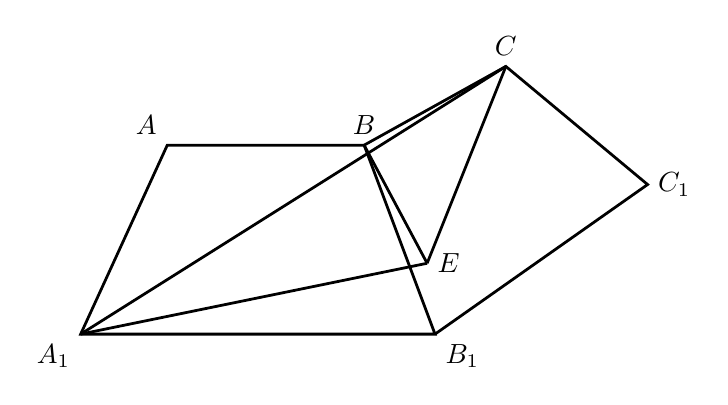
\begin{tikzpicture}[line width=1pt]
\coordinate (A) at (1.6,2.9);
\coordinate (B) at (4.1,2.9);
\coordinate (C) at (5.9,3.9);
\coordinate (C1) at (7.7,2.4);
\coordinate (E) at (4.9,1.4);
\coordinate (B1) at (5.0,0.5);
\coordinate (A1) at (0.5,0.5);

\draw (A) -- (B) -- (B1) -- (A1) -- cycle;
\draw (B) -- (C) -- (C1) -- (B1);
\draw (A1) -- (C);
\draw (A1) -- (E);
\draw (C) -- (E);
\draw (B) -- (E);

\node[above left] at (A) {$A$};
\node[above] at (B) {$B$};
\node[above] at (C) {$C$};
\node[right] at (C1) {$C_1$};
\node[right] at (E) {$E$};
\node[below right] at (B1) {$B_1$};
\node[below left] at (A1) {$A_1$};
\end{tikzpicture}
\end{document}
